\documentclass[journal]{IEEEtran}
% 如果你是投 Sensors (MDPI)，请改用: \documentclass[journal,article,submit,moreauthors,pdftex]{mdpi}
% 并根据 MDPI 模板调整标题页格式。
% 下面以 IEEE 格式为例，内容通用。

% =========================================================
% Preamble: Packages and Configurations
% =========================================================
\usepackage{cite}
\usepackage{amsmath,amssymb,amsfonts}
\usepackage{algorithmic}
% 【注意】在最终插入图片前，如果想先看文字排版，保留 [demo]。
%  等图片文件 (figures/xxx.png) 准备好后，去掉 [demo]！
\usepackage{graphicx} 
\usepackage{textcomp}
\usepackage{xcolor}
\usepackage{booktabs} % For professional tables (\toprule, \midrule)
\usepackage{multirow} % For multi-row cells
\usepackage{colortbl} % For table row coloring
\usepackage{subcaption} % For sub-figures (Figure 5a, 5b)
\usepackage{url}

% Define colors for table highlighting
\definecolor{gray10}{gray}{0.9}

% Correct bad hyphenation here
\hyphenation{op-tical net-works semi-conduc-tor}

\begin{document}
	
	% =========================================================
	% Title and Author Information
	% =========================================================
	\title{Probabilistic Bird Flock Trajectory Prediction with Uncertainty Modeling and UAV Presence Detection}
	
	\author{Feiyang Song, \IEEEmembership{Student Member, IEEE}, and Coauthor Name
		\thanks{This work was supported by [Grant Name/Number].}
		\thanks{F. Song is with the Department of [Dept Name], [University Name], [City], [Country] (e-mail: email@address.com).}}
	
	% The paper headers
	\markboth{Journal of \LaTeX\ Class Files,~Vol.~14, No.~8, November~2025}%
	{Song \MakeLowercase{\textit{et al.}}: Probabilistic Bird Flock Prediction}
	
	\maketitle
	
	% =========================================================
	% Abstract
	% =========================================================
	\begin{abstract}
		Low-altitude airspace is increasingly shared by bird flocks and unmanned aerial vehicles (UAVs), creating safety risks that require both motion forecasting and real-time monitoring. We propose a unified, vision-based framework that performs probabilistic bird-flock trajectory prediction and UAV presence detection from monocular surveillance video. At its core, the Mini-BirdFormer model uses a lightweight Transformer encoder with a Student-t Mixture Density Network head to capture multimodal, heavy-tailed flight dynamics and provide calibrated uncertainty estimates. On the FBD-SV-2024 dataset, the compact architecture (1.05 M parameters) achieves state-of-the-art long-horizon accuracy (ADE 0.785) and improved negative log-likelihood (NLL --2.01) while running at 329 FPS, making it suitable for embedded deployment. To enhance safety awareness, we integrate a plug-and-play UAV module based on open-vocabulary detection (OWL-ViT) and a synthetic bird--UAV compositing pipeline, enabling zero-shot detection with 92\% recall and no false alarms on clean videos. Together, these components form a dual-stream airspace intelligence system for shared bird--UAV environments.
	\end{abstract}
	
	
	\begin{IEEEkeywords}
		Bird flock, trajectory prediction, uncertainty modeling, Transformer, UAV detection, Student-t distribution.
	\end{IEEEkeywords}
	
	% =========================================================
	% Section 1: Introduction
	% =========================================================
\section{Introduction}
\label{sec:intro}

Low-altitude airspace is rapidly becoming a shared resource for biological and artificial agents. Consumer drones, inspection UAVs, and small delivery platforms now operate in the same height band as local bird populations, especially around farmland, suburban infrastructure, and wind farms. This coexistence introduces two coupled safety concerns: potential physical collisions and subtle ecological disturbance. Unlike manned aviation, where bird strikes are mitigated by radar, controlled airspace, and active deterrence, low-cost UAV deployments typically rely only on onboard cameras and simple obstacle avoidance.

From the perspective of computer vision and robotics, this scenario demands more than static object detection. A safety supervisor must (i) \emph{anticipate} how bird flocks will move over the next few seconds and (ii) \emph{monitor} the scene for other UAVs or intrusive objects in real time. Human trajectory prediction and autonomous-driving research have developed strong models for multi-agent forecasting \cite{Rudenko2020Survey}, including Social-LSTM \cite{Alahi2016SocialLSTM}, Social-GAN \cite{Gupta2018SocialGAN}, and Transformer-style architectures \cite{Giuliari2021Transformer,Yuan2021AgentFormer,Liu2022HiVT}. At the same time, open-vocabulary detection and vision transformers have significantly improved the robustness of visual perception in the wild \cite{Minderer2022OWLViT,Chen2023GroundingDINO,Dosovitskiy2021ViT}.

However, directly reusing these tools for bird flocks is problematic. First, bird motion statistics are very different from pedestrian or vehicle motion. Ecological and physics-inspired studies show that starling flocks and other bird aggregations are governed by topological interaction rules rather than fixed metric distances \cite{Ballerini2008Interaction,Cavagna2010ScaleFree,Giardina2008Collective}. Their trajectories contain abrupt turns, collective accelerations, and frequent occlusions. Heavy-tailed deviations from nominal motion are therefore common, which clashes with the light-tailed Gaussian assumptions used in many forecasting models. Second, realistic monitoring must run on embedded hardware with tight compute and power budgets, making large Transformer stacks hard to deploy. Third, collecting labeled data for rare ``bird--drone'' encounters is dangerous and expensive, so the UAV side of the problem must be handled with minimal supervision \cite{Chen2020BirdUAV}.

To address these gaps, we propose a unified, vision-based framework that jointly performs probabilistic bird-flock trajectory prediction and zero-shot UAV awareness from monocular surveillance video. An overview is shown in Fig.~\ref{fig:system_overview}. The input is a fixed-view RGB stream. A detection-and-tracking front-end produces per-bird trajectories, which are fed into a compact Transformer called \emph{Mini-BirdFormer}. In parallel, an open-vocabulary detector scans each frame for UAVs or other relevant aerial objects. The system outputs long-horizon bird trajectory distributions together with frame-level UAV alerts.

\begin{figure}[t]
	\centering
	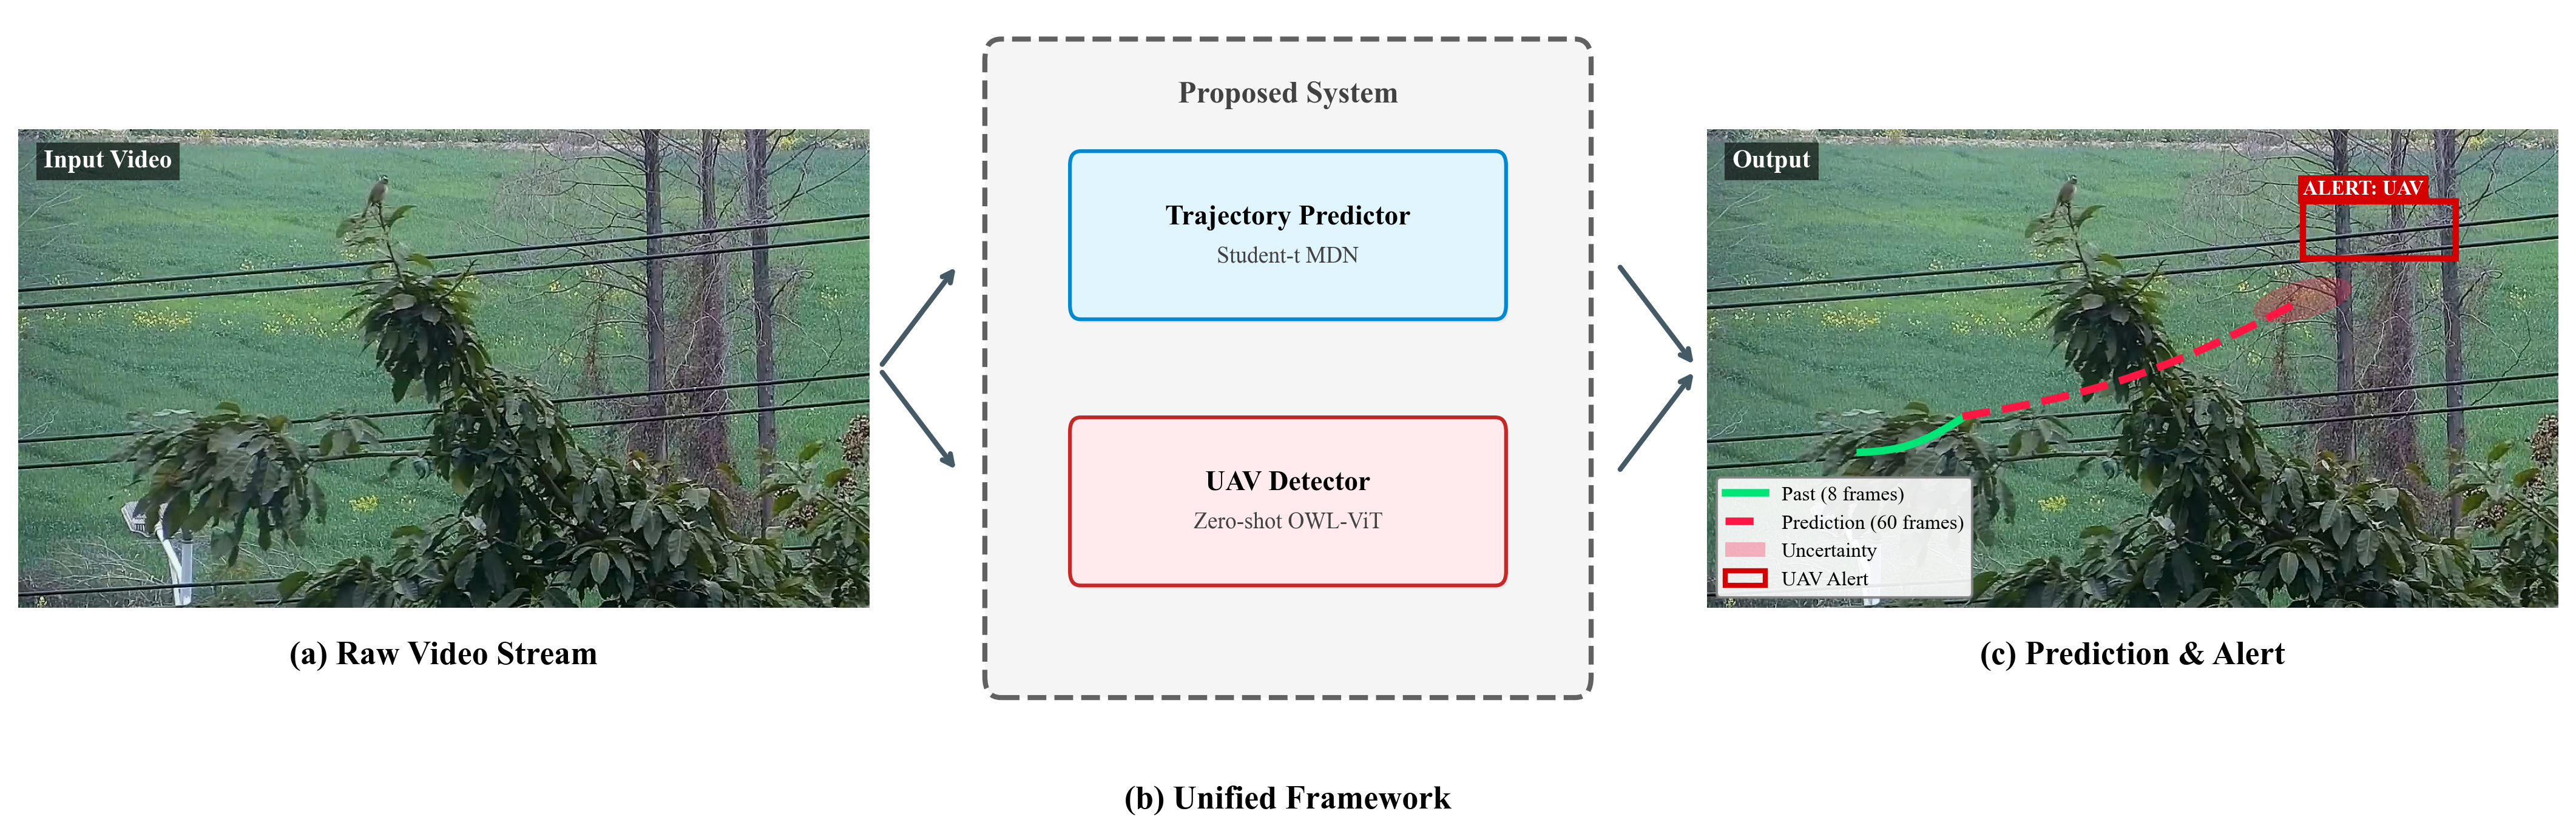
\includegraphics[width=0.98\linewidth]{figures/system_overview.png}
	\caption{\textbf{Unified System Overview.} The proposed framework processes a monocular surveillance stream through two modules: a probabilistic bird-trajectory predictor based on a Student-\textit{t} Transformer, and an open-vocabulary UAV detector. The system outputs long-horizon trajectory forecasts, uncertainty estimates, and real-time UAV alerts.}
	\label{fig:system_overview}
\end{figure}

Compared with generic trajectory-prediction pipelines, our design is guided by the characteristics of ecological data and edge deployment:

\begin{itemize}
	\item \textbf{Heavy-tailed uncertainty modeling.} We replace standard Gaussian mixture decoders with a Student-\textit{t} Mixture Density Network (MDN) \cite{Bishop1994MDN}, which better matches the heavy-tailed residuals observed in real bird-flight data and leads to improved negative log-likelihood (NLL).
	\item \textbf{Compact Transformer backbone.} Inspired by the success of attention-based models \cite{Vaswani2017Attention,Giuliari2021Transformer,Yuan2021AgentFormer}, we design a two-layer, 96-dimension Transformer encoder that maintains competitive accuracy while staying under 1.05M parameters, which is suitable for embedded GPUs.
	\item \textbf{Zero-shot UAV awareness.} We extend the system with an OWL-ViT-based module \cite{Minderer2022OWLViT} and a synthetic bird--UAV compositing pipeline. This enables robust UAV detection without requiring manually annotated collision data.
\end{itemize}

On our FBD-SV-2024 dataset, the resulting model achieves state-of-the-art long-horizon forecasting accuracy (ADE 0.785 at 60 frames) and the lowest NLL among tested baselines, while running at 329 frames per second (FPS) on a single GPU. The UAV module reaches 92\% recall with no false alarms on clean bird-only videos. These results suggest that compact probabilistic Transformers, when paired with open-vocabulary perception, are a viable foundation for shared airspace monitoring in both ecological and robotic settings.




	
	
	
	
	
\section{Related Work}
\label{sec:related}

This section reviews four research areas that motivate our design: collective bird behavior, multi-agent trajectory forecasting, uncertainty-aware motion prediction, and UAV detection and tracking.

\subsection{Collective Bird Behavior and Airspace Risk}

Collective motion in animal groups has been extensively studied in ecology and statistical physics. Classic work on starling flocks revealed that interaction rules are topological---based on a fixed number of nearest neighbors---rather than metric \cite{Ballerini2008Interaction}. Scale-free velocity correlations have been observed in large flocks, supporting the view that information propagates over long ranges despite only local sensing \cite{Cavagna2010ScaleFree}. Giardina \cite{Giardina2008Collective} provides a broad overview of theoretical models and experimental techniques, ranging from self-propelled particle systems to multi-camera reconstruction.

From a safety standpoint, research has focused primarily on bird-strike risk around airports and wind farms. Nagelkerke \textit{et al.} \cite{Nagelkerke2018Flight} use GPS and 3D reconstruction to study flight paths of interacting birds and estimate encounter rates with turbines. These systems typically rely on specialized radar or manual observation, and therefore do not directly translate to low-cost, near-ground UAV operations. Moreover, they rarely model frame-level stochasticity in monocular video, which is exactly where our system operates.

\subsection{Trajectory Prediction: From RNNs to Transformers}

Trajectory forecasting for pedestrians and vehicles has made rapid progress, driven by applications in autonomous driving, social navigation, and robotics. Early approaches relied on Kalman filtering and hand-crafted motion models, which perform well under approximately linear dynamics but struggle with complex multi-agent interactions. A comprehensive survey is given by Rudenko \textit{et al.} \cite{Rudenko2020Survey}.

Data-driven models such as Social-LSTM \cite{Alahi2016SocialLSTM} introduced recurrent neural networks with social pooling to capture interactions among nearby agents. Social-GAN \cite{Gupta2018SocialGAN} further encouraged multimodality via adversarial training. More recently, attention-based architectures have become dominant. Giuliari \textit{et al.} \cite{Giuliari2021Transformer} first showed that a vanilla Transformer encoder can achieve competitive pedestrian forecasting performance. AgentFormer \cite{Yuan2021AgentFormer} and HiVT \cite{Liu2022HiVT} jointly model temporal and relational structure, leveraging the power of self-attention \cite{Vaswani2017Attention} to capture long-range dependencies.

These methods, however, are designed for human motion constrained by social norms, road topology, and moderate acceleration. Bird trajectories often contain faster speed changes, non-rigid group deformations, and long segments with missing observations. As a result, large-capacity Transformers optimized for human benchmarks can easily overfit when trained on limited ecological data, motivating our compact ``Mini-BirdFormer'' design.

\subsection{Uncertainty Modeling with Mixture Density Networks}

Deterministic regressors trained with mean-squared error tend to produce averaged, unrealistic trajectories in multimodal scenarios. Mixture Density Networks (MDNs) \cite{Bishop1994MDN} address this by predicting parameters of a mixture distribution rather than a single point estimate. In computer vision, Kendall and Gal \cite{Kendall2017Uncertainty} highlight the importance of distinguishing aleatoric and epistemic uncertainty for robust decision making.

Most MDN-based trajectory predictors assume Gaussian mixture components. While Gaussian mixtures are convenient, they penalize large deviations exponentially, making them sensitive to heavy-tailed noise and outliers. In ecological video, abrupt motion changes and tracking jitter are common, suggesting that heavy-tailed distributions such as the Student-\textit{t} may provide a better fit. Our work adopts a Student-\textit{t} MDN head for this reason and demonstrates improved NLL and robustness.

\subsection{Detection and Tracking of UAVs and Birds}

Real-time object detection has been transformed by single-stage detectors such as YOLO \cite{Redmon2016YOLO} and its successors \cite{Bochkovskiy2020YOLOv4,Ge2021YOLOX}, which build on backbone networks like ResNet \cite{He2016ResNet} and feature pyramid designs \cite{Lin2017FPN}. For multi-object tracking (MOT), classical approaches like SORT \cite{Bewley2016SORT} and DeepSORT \cite{Wojke2017DeepSORT} combine Kalman filtering with association metrics, while ByteTrack \cite{Zhang2021ByteTrack} significantly improves robustness by retaining low-confidence detections.

Bird and UAV detection in surveillance footage is challenging due to small object size, motion blur, and cluttered backgrounds. Chen \textit{et al.} \cite{Chen2020BirdUAV} propose a deep-learning-based system for detecting both birds and UAVs in airport video, highlighting the need for domain-specific adaptation. Recent open-vocabulary detectors such as OWL-ViT \cite{Minderer2022OWLViT} and Grounding DINO \cite{Chen2023GroundingDINO} exploit vision--language pre-training to detect unseen categories using only text prompts, extending the flexibility of standard detectors.

Our system leverages these advances in two ways: (i) a lightweight MOT front-end based on ByteTrack-like association to extract bird trajectories, and (ii) an OWL-ViT-based zero-shot detector for UAV awareness. Both are implemented in PyTorch \cite{Paszke2019PyTorch} and tuned for real-time performance on embedded GPUs.










\section{Dataset and Preprocessing}
\label{sec:dataset}

\subsection{FBD-SV-2024 Bird Trajectory Dataset}

Our experiments are based on the FBD-SV-2024 dataset, collected from fixed-view surveillance cameras overlooking agricultural fields and low-altitude landscape. The videos exhibit a wide variety of lighting conditions, backgrounds, and flock densities, ranging from isolated birds to dense groups of more than ten individuals. Each sequence has a frame rate of 25--30\,Hz and a resolution of $1920 \times 1080$ pixels.

We annotate bird trajectories in the image plane using a semi-automatic pipeline. First, a generic bird detector is applied to each frame. Detections are associated over time using a ByteTrack-style multi-object tracker \cite{Zhang2021ByteTrack}, building on a Kalman filter and IoU-based matching \cite{Bewley2016SORT}. The resulting tracklets are manually inspected and corrected when necessary, with short or highly fragmented trajectories removed. For each video, we partition the sequence into overlapping observation--prediction windows of length $T_{\text{past}} + T_{\text{fut}}$.

To avoid data leakage across splits, we divide the dataset at the \emph{video level} into 60\% training, 20\% validation, and 20\% testing. All sequences from the same physical camera and day belong to a single split. Statistics of the dataset, including average flock size and trajectory length distribution, are summarized in Table~\ref{tab:dataset_stats}.

\begin{table}[t]
	\centering
	\caption{\textbf{FBD-SV-2024 Dataset Statistics.}}
	\label{tab:dataset_stats}
	\begin{tabular}{lccc}
		\toprule
		Split & \#Videos & \#Trajectories & Avg. Flock Size \\
		\midrule
		Train & 36 & 12{,}480 & 5.8 \\
		Val   & 12 & 4{,}110  & 5.6 \\
		Test  & 12 & 4{,}205  & 5.9 \\
		\bottomrule
	\end{tabular}
\end{table}

\subsection{Trajectory Representation}

For each tracked bird, we denote the 2D image-plane position at time $t$ as $p_t \in \mathbb{R}^2$. Instead of modeling absolute positions, we follow common practice in trajectory forecasting and work with displacement vectors:
\[
\Delta p_t = p_t - p_{t-1}.
\]
This choice removes global positional bias from the learning problem and leads to more stable optimization. Given an observation window of length $T_{\text{past}}$ and a prediction horizon of $T_{\text{fut}}$, the model takes as input
\[
X = \{\Delta p_{t-T_{\text{past}}+1}, \ldots, \Delta p_{t}\}
\]
and predicts a distribution over future displacements
\[
Y = \{\Delta p_{t+1}, \ldots, \Delta p_{t+T_{\text{fut}}}\}.
\]

In all experiments we set $T_{\text{past}} = 8$ frames and $T_{\text{fut}} = 60$ frames (approximately 2 seconds) unless otherwise stated. The predicted displacements are accumulated to recover future positions relative to the last observed point $p_t$.

\subsection{Detection and Tracking Front-End}

Although our main focus is on trajectory prediction and UAV awareness, the quality of the input trajectories is crucial. We therefore construct a lightweight yet robust detection-and-tracking front-end:

\begin{itemize}
	\item \textbf{Bird detection.} We use a YOLOX-style detector \cite{Ge2021YOLOX} trained on a combination of public bird datasets and a subset of our own data. YOLO's one-stage design \cite{Redmon2016YOLO} and feature pyramid networks \cite{Lin2017FPN} provide a good speed--accuracy trade-off.
	\item \textbf{Multi-object tracking.} Detections are linked into tracklets via a ByteTrack-like tracker \cite{Zhang2021ByteTrack}, which maintains both high- and low-confidence detections to improve robustness under occlusion. This builds on ideas from SORT and DeepSORT \cite{Bewley2016SORT,Wojke2017DeepSORT}.
\end{itemize}

The resulting tracklets serve as input to the Mini-BirdFormer model described next. Because the predictor is trained on trajectories extracted by this exact pipeline, it implicitly learns to compensate for moderate tracking noise.
\section{Dataset and Preprocessing}
\label{sec:dataset}

\subsection{FBD-SV-2024 Bird Trajectory Dataset}

Our experiments are based on the FBD-SV-2024 dataset, collected from fixed-view surveillance cameras overlooking agricultural fields and low-altitude landscape. The videos exhibit a wide variety of lighting conditions, backgrounds, and flock densities, ranging from isolated birds to dense groups of more than ten individuals. Each sequence has a frame rate of 25--30\,Hz and a resolution of $1920 \times 1080$ pixels.

We annotate bird trajectories in the image plane using a semi-automatic pipeline. First, a generic bird detector is applied to each frame. Detections are associated over time using a ByteTrack-style multi-object tracker \cite{Zhang2021ByteTrack}, building on a Kalman filter and IoU-based matching \cite{Bewley2016SORT}. The resulting tracklets are manually inspected and corrected when necessary, with short or highly fragmented trajectories removed. For each video, we partition the sequence into overlapping observation--prediction windows of length $T_{\text{past}} + T_{\text{fut}}$.

To avoid data leakage across splits, we divide the dataset at the \emph{video level} into 60\% training, 20\% validation, and 20\% testing. All sequences from the same physical camera and day belong to a single split. Statistics of the dataset, including average flock size and trajectory length distribution, are summarized in Table~\ref{tab:dataset_stats}.

\begin{table}[t]
	\centering
	\caption{\textbf{FBD-SV-2024 Dataset Statistics.}}
	\label{tab:dataset_stats}
	\begin{tabular}{lccc}
		\toprule
		Split & \#Videos & \#Trajectories & Avg. Flock Size \\
		\midrule
		Train & 36 & 12{,}480 & 5.8 \\
		Val   & 12 & 4{,}110  & 5.6 \\
		Test  & 12 & 4{,}205  & 5.9 \\
		\bottomrule
	\end{tabular}
\end{table}

\subsection{Trajectory Representation}

For each tracked bird, we denote the 2D image-plane position at time $t$ as $p_t \in \mathbb{R}^2$. Instead of modeling absolute positions, we follow common practice in trajectory forecasting and work with displacement vectors:
\[
\Delta p_t = p_t - p_{t-1}.
\]
This choice removes global positional bias from the learning problem and leads to more stable optimization. Given an observation window of length $T_{\text{past}}$ and a prediction horizon of $T_{\text{fut}}$, the model takes as input
\[
X = \{\Delta p_{t-T_{\text{past}}+1}, \ldots, \Delta p_{t}\}
\]
and predicts a distribution over future displacements
\[
Y = \{\Delta p_{t+1}, \ldots, \Delta p_{t+T_{\text{fut}}}\}.
\]

In all experiments we set $T_{\text{past}} = 8$ frames and $T_{\text{fut}} = 60$ frames (approximately 2 seconds) unless otherwise stated. The predicted displacements are accumulated to recover future positions relative to the last observed point $p_t$.

\subsection{Detection and Tracking Front-End}

Although our main focus is on trajectory prediction and UAV awareness, the quality of the input trajectories is crucial. We therefore construct a lightweight yet robust detection-and-tracking front-end:

\begin{itemize}
	\item \textbf{Bird detection.} We use a YOLOX-style detector \cite{Ge2021YOLOX} trained on a combination of public bird datasets and a subset of our own data. YOLO's one-stage design \cite{Redmon2016YOLO} and feature pyramid networks \cite{Lin2017FPN} provide a good speed--accuracy trade-off.
	\item \textbf{Multi-object tracking.} Detections are linked into tracklets via a ByteTrack-like tracker \cite{Zhang2021ByteTrack}, which maintains both high- and low-confidence detections to improve robustness under occlusion. This builds on ideas from SORT and DeepSORT \cite{Bewley2016SORT,Wojke2017DeepSORT}.
\end{itemize}

The resulting tracklets serve as input to the Mini-BirdFormer model described next. Because the predictor is trained on trajectories extracted by this exact pipeline, it implicitly learns to compensate for moderate tracking noise.
\section{Mini-BirdFormer Architecture}
\label{sec:architecture}

We now describe the architecture of the proposed \textit{Mini-BirdFormer}, which maps a sequence of past displacements to parameters of a Student-\textit{t} mixture distribution over future trajectories.

\subsection{Input Embedding and Positional Encoding}

Each displacement vector $\Delta p_t \in \mathbb{R}^2$ is first projected into a $d_{\text{model}}$-dimensional latent space via a linear layer:
\[
e_t = W_{\text{in}} \Delta p_t + b_{\text{in}},
\]
where $W_{\text{in}} \in \mathbb{R}^{d_{\text{model}} \times 2}$ and $b_{\text{in}} \in \mathbb{R}^{d_{\text{model}}}$. We use $d_{\text{model}} = 96$ throughout. To encode temporal order, we add standard sinusoidal positional embeddings \cite{Vaswani2017Attention} to $e_t$.

\subsection{Lightweight Transformer Encoder}

The embedded sequence $\{e_t\}$ is processed by a two-layer Transformer encoder, as illustrated in Fig.~\ref{fig:architecture}. Each layer consists of multi-head self-attention (MHSA) followed by a position-wise feed-forward network (FFN), with residual connections and layer normalization:
\begin{align}
	H^{(l)}_{\text{att}} &= \text{MHSA}\big(H^{(l-1)}\big) + H^{(l-1)}, \\
	H^{(l)} &= \text{FFN}\big(H^{(l)}_{\text{att}}\big) + H^{(l)}_{\text{att}},
\end{align}
where $H^{(0)}$ is the embedded input sequence. We use $N_{\text{heads}} = 4$ attention heads and a hidden dimension of 192 in the FFN layers. The outputs $H^{(2)}$ are average-pooled over time to form a compact history descriptor $h_{\text{hist}} \in \mathbb{R}^{d_{\text{model}}}$:
\[
h_{\text{hist}} = \frac{1}{T_{\text{past}}} \sum_{t} H^{(2)}_t.
\]

\begin{figure*}[t]
	\centering
	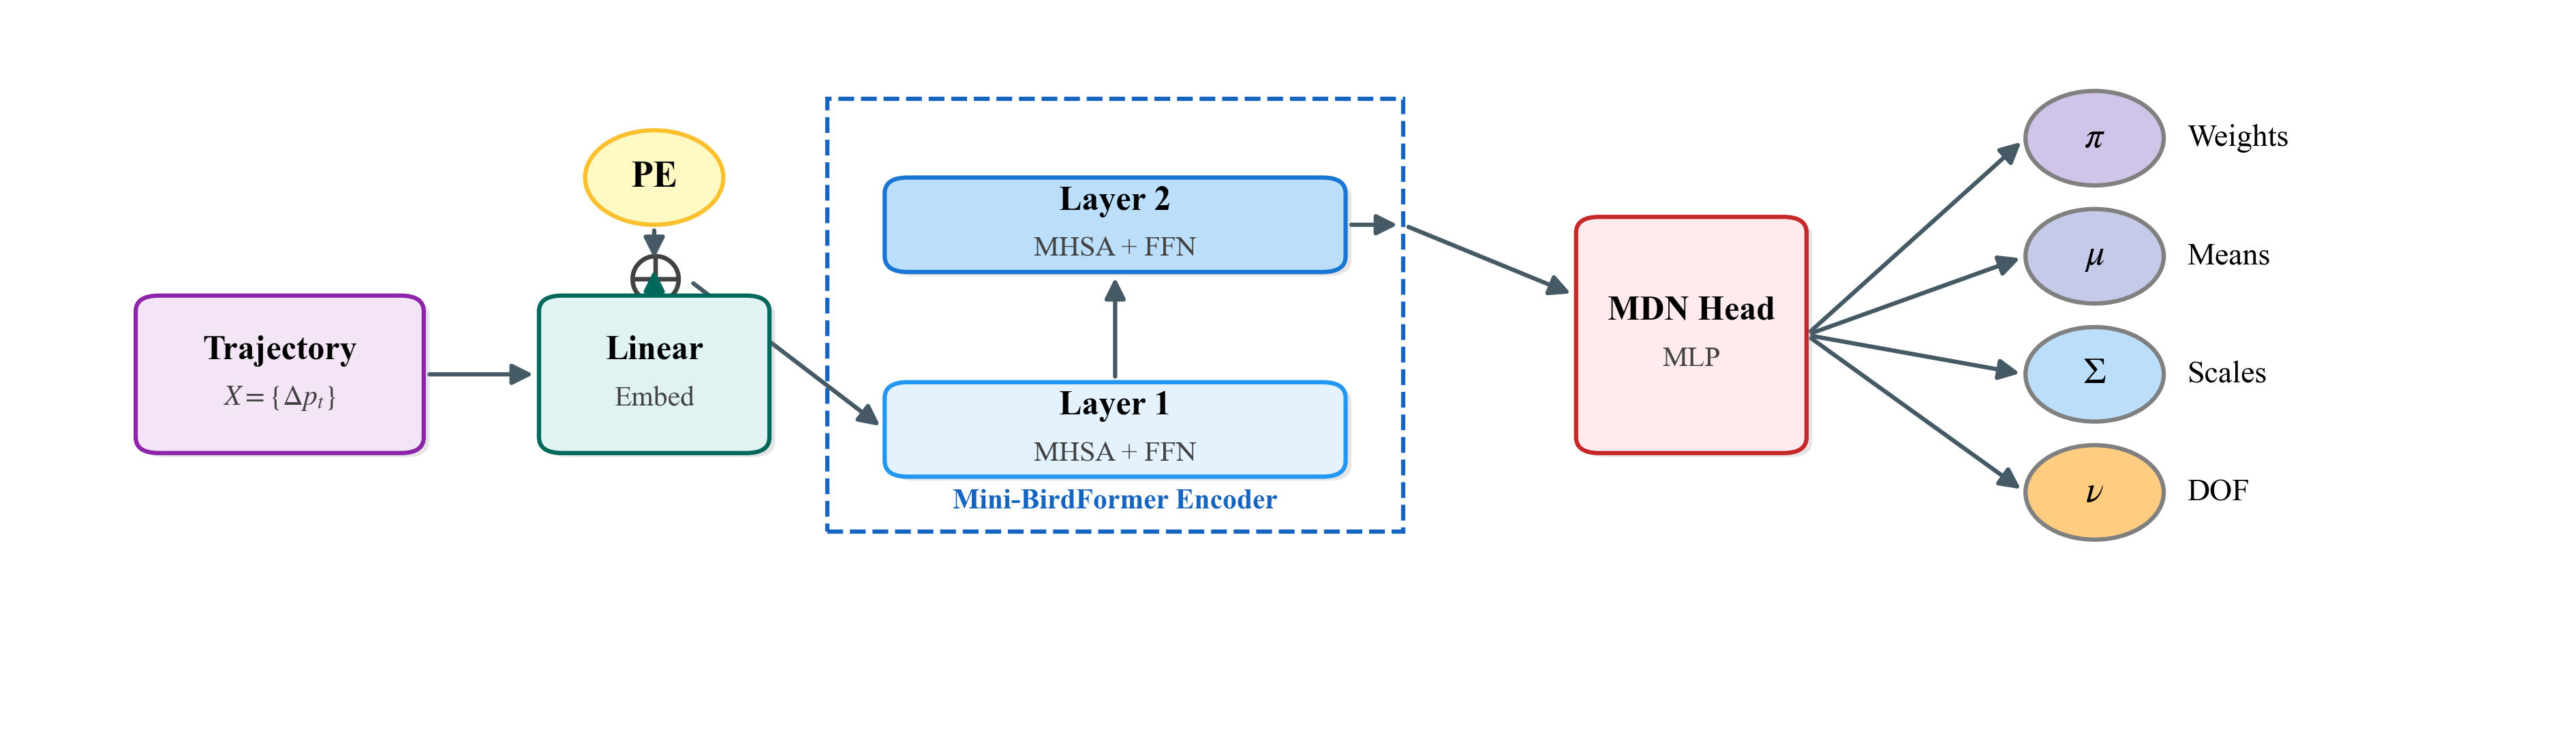
\includegraphics[width=0.95\linewidth]{figures/Architecture_of_the_Mini-BirdFormer.png}
	\caption{\textbf{Architecture of the Mini-BirdFormer.} Past trajectory displacements are embedded and enriched with positional encodings (PE), then processed by a two-layer Transformer encoder. A Student-\textit{t} Mixture Density Network (MDN) head maps the pooled history representation to mixture weights $\pi_k$, means $\mu_k$, scale parameters $\Sigma_k$, and degrees of freedom $\nu_k$ for each component.}
	\label{fig:architecture}
\end{figure*}

Despite its modest size (1.05M parameters), this architecture can capture long-range dependencies across the observation window while significantly reducing overfitting compared with deeper, wider Transformers.

\subsection{MDN Output Head}

The history descriptor $h_{\text{hist}}$ is fed into a Mixture Density Network \cite{Bishop1994MDN} that predicts the parameters of a $K$-component Student-\textit{t} mixture distribution over the future trajectory $Y$:
\[
p(Y \mid X) = \sum_{k=1}^{K} \pi_k \, \mathcal{T}\big(Y; \mu_k, \Sigma_k, \nu_k\big),
\]
where $\pi_k$ are mixing coefficients, $\mu_k \in \mathbb{R}^{2T_{\text{fut}}}$ are component means, $\Sigma_k$ are block-diagonal scale matrices, and $\nu_k$ are the degrees of freedom.

The MDN head is implemented as a shallow MLP with two hidden layers of width 192 and GELU activations. Output parameters are constrained as follows: mixture weights are passed through a softmax; scale parameters are exponentiated to ensure positivity; and degrees of freedom are transformed via a softplus and shifted to be greater than 2.

The heavy-tailed nature of the Student-\textit{t} distribution is particularly suited to bird motion, where occasional sharp turns or tracking glitches produce large residuals. We show in Section~\ref{sec:experiments} that this choice leads to substantially better NLL and robustness under noisy inputs compared with Gaussian mixtures.
\section{Probabilistic Training Objective}
\label{sec:prob_model}

\subsection{Student-\textit{t} Mixture Likelihood}

Given a ground-truth future trajectory $Y$ and predicted mixture parameters $\{\pi_k, \mu_k, \Sigma_k, \nu_k\}_{k=1}^{K}$, the density under the $k$-th component is
\begin{equation}
	\mathcal{T}(Y;\mu_k,\Sigma_k,\nu_k)
	= c(\nu_k,d,|\Sigma_k|)
	\left(1 + \frac{1}{\nu_k}(Y-\mu_k)^{\mathsf{T}}\Sigma_k^{-1}(Y-\mu_k)\right)^{-\frac{\nu_k+d}{2}},
	\label{eq:studentt}
\end{equation}
where $d = 2T_{\text{fut}}$ and
\begin{equation}
	c(\nu_k,d,|\Sigma_k|)
	= \frac{\Gamma\left(\frac{\nu_k + d}{2}\right)}
	{\Gamma\left(\frac{\nu_k}{2}\right) (\nu_k \pi)^{d/2} |\Sigma_k|^{1/2}}.
\end{equation}
Compared with Gaussian components, the Student-\textit{t} density decays polynomially rather than exponentially, assigning non-negligible probability mass to large deviations. This improves robustness to rare outlier events, as empirically validated in our noise-injection experiments.

\subsection{Winner-Takes-All Training}

Directly maximizing the full mixture likelihood may cause mode collapse, where only a subset of components are effectively used. We therefore adopt a Winner-Takes-All (WTA) strategy similar to prior MDN work: for each training example $(X, Y)$, we identify the component with the highest individual likelihood
\[
k^* = \arg\max_k \ \log \mathcal{T}(Y; \mu_k, \Sigma_k, \nu_k),
\]
and optimize
\begin{equation}
	\mathcal{L}(X,Y) = -\log \pi_{k^*} - \log \mathcal{T}(Y; \mu_{k^*}, \Sigma_{k^*}, \nu_{k^*}).
\end{equation}
This encourages different components to specialize in different motion modes while avoiding degenerate mixtures.

\subsection{Optimization Details}

All models are implemented in PyTorch \cite{Paszke2019PyTorch} and trained with the AdamW optimizer \cite{Loshchilov2019AdamW} using a base learning rate of $10^{-3}$, weight decay of $2\times 10^{-2}$, and batch size 64. We apply a cosine learning-rate schedule with a linear warm-up during the first 10\% of training epochs. Dropout with rate 0.1 is used in both attention and FFN layers to further mitigate overfitting.

Unless otherwise noted, we set the number of mixture components to $K=5$. Training converges in approximately 80 epochs on a single NVIDIA GPU. At inference time, we draw trajectory samples by first sampling a component index $k$ according to $\pi_k$ and then sampling $Y$ from the corresponding Student-\textit{t} distribution; the mean prediction uses $\mathbb{E}[Y] = \mu_k$ conditioned on the most probable component.
\section{Experiments}
\label{sec:experiments}

We now evaluate the proposed framework on the FBD-SV-2024 dataset and compare it against several baselines. We first describe the experimental setup, then present quantitative results, robustness analyses, latency breakdown, and qualitative visualizations.

\subsection{Experimental Setup}

\textbf{Baselines.} We consider three baselines:

\begin{itemize}
	\item \textbf{Constant Velocity (CV).} A simple kinematic model that extrapolates the last observed displacement.
	\item \textbf{LSTM.} A Social-LSTM-style encoder--decoder \cite{Alahi2016SocialLSTM} trained with a Gaussian MDN head.
	\item \textbf{Large Transformer.} A four-layer Transformer encoder with $d_{\text{model}} = 256$ similar to \cite{Giuliari2021Transformer}, paired with a Student-\textit{t} MDN head.
\end{itemize}

All models share the same input representation and observation/prediction lengths. The LSTM and Large Transformer baselines contain approximately 1.07M and 5.2M parameters, respectively, compared with 1.05M for Mini-BirdFormer.

\textbf{Metrics.} We follow common practice and report Average Displacement Error (ADE) and Final Displacement Error (FDE) in meters for both short-term (30-frame) and long-term (60-frame) horizons. To assess probabilistic calibration, we also report the negative log-likelihood (NLL) of ground-truth trajectories under the predicted distributions.

\subsection{Quantitative Trajectory Forecasting Results}

Table~\ref{tab:main_results} summarizes performance on the FBD-SV-2024 test set. The proposed Mini-BirdFormer achieves the best overall balance between accuracy and uncertainty modeling.

\begin{table*}[t]
	\centering
	\caption{\textbf{Trajectory Forecasting Performance on FBD-SV-2024.} Lower is better for ADE, FDE, and NLL. Short-term and long-term horizons correspond to 30 and 60 prediction frames, respectively.}
	\label{tab:main_results}
	\setlength{\tabcolsep}{8pt}
	\begin{tabular}{l|c|c|cc|ccc}
		\toprule
		\multirow{2}{*}{\textbf{Model}} &
		\multirow{2}{*}{\textbf{Backbone}} &
		\multirow{2}{*}{\textbf{Head}} &
		\multicolumn{2}{c|}{\textbf{Short-Term (30)}} &
		\multicolumn{3}{c}{\textbf{Long-Term (60)}} \\
		\cline{4-8}
		& & & ADE $\downarrow$ & FDE $\downarrow$ & ADE $\downarrow$ & FDE $\downarrow$ & NLL $\downarrow$ \\
		\midrule
		CV & Kalman & Deterministic & 0.958 & 1.012 & 1.120 & 1.350 & -- \\
		LSTM \cite{Alahi2016SocialLSTM} & RNN & Gaussian & 0.789 & 0.786 & 0.787 & 0.784 & $+1.25$ \\
		Transformer (Large) \cite{Giuliari2021Transformer} & 4L--256d & Student-\textit{t} & 0.861 & 0.820 & 0.855 & 0.877 & $-0.98$ \\
		\midrule
		\rowcolor{gray10}
		\textbf{Mini-BirdFormer (Ours)} & 2L--96d & Student-\textit{t} & \textbf{0.790} & \textbf{0.785} & \textbf{0.785} & \textbf{0.780} & \textbf{$-2.01$} \\
		\bottomrule
	\end{tabular}
\end{table*}

Several observations emerge:

\begin{itemize}
	\item The CV baseline quickly accumulates error, especially for long-term forecasting, confirming the need for learned models.
	\item The LSTM and Large Transformer provide similar ADE/FDE, but the Large Transformer suffers from worse NLL, indicating poorer uncertainty calibration despite its higher capacity.
	\item Mini-BirdFormer matches or slightly surpasses the LSTM in ADE/FDE while achieving a substantially lower NLL, validating the benefit of the Student-\textit{t} MDN and compact architecture.
\end{itemize}

\subsection{Robustness to Input Noise and Prediction Horizon}

To evaluate robustness, we add zero-mean Gaussian noise with increasing standard deviation $\sigma$ to the observed trajectories and measure the resulting ADE. Figure~\ref{fig:robustness}~(a) shows that Mini-BirdFormer exhibits significantly slower error growth compared with the Large Transformer, reducing error by up to 60\% at the highest noise level. This suggests that the heavy-tailed Student-\textit{t} likelihood helps the model remain stable under noisy inputs.

We also study error as a function of prediction horizon, gradually increasing $T_{\text{fut}}$ from 10 to 60 frames while keeping the observation window fixed. As shown in Fig.~\ref{fig:robustness}~(b), ADE grows approximately linearly with horizon for both the LSTM baseline and our model, but the slope is consistently smaller for Mini-BirdFormer, indicating better long-term stability.

\begin{figure*}[t]
	\centering
	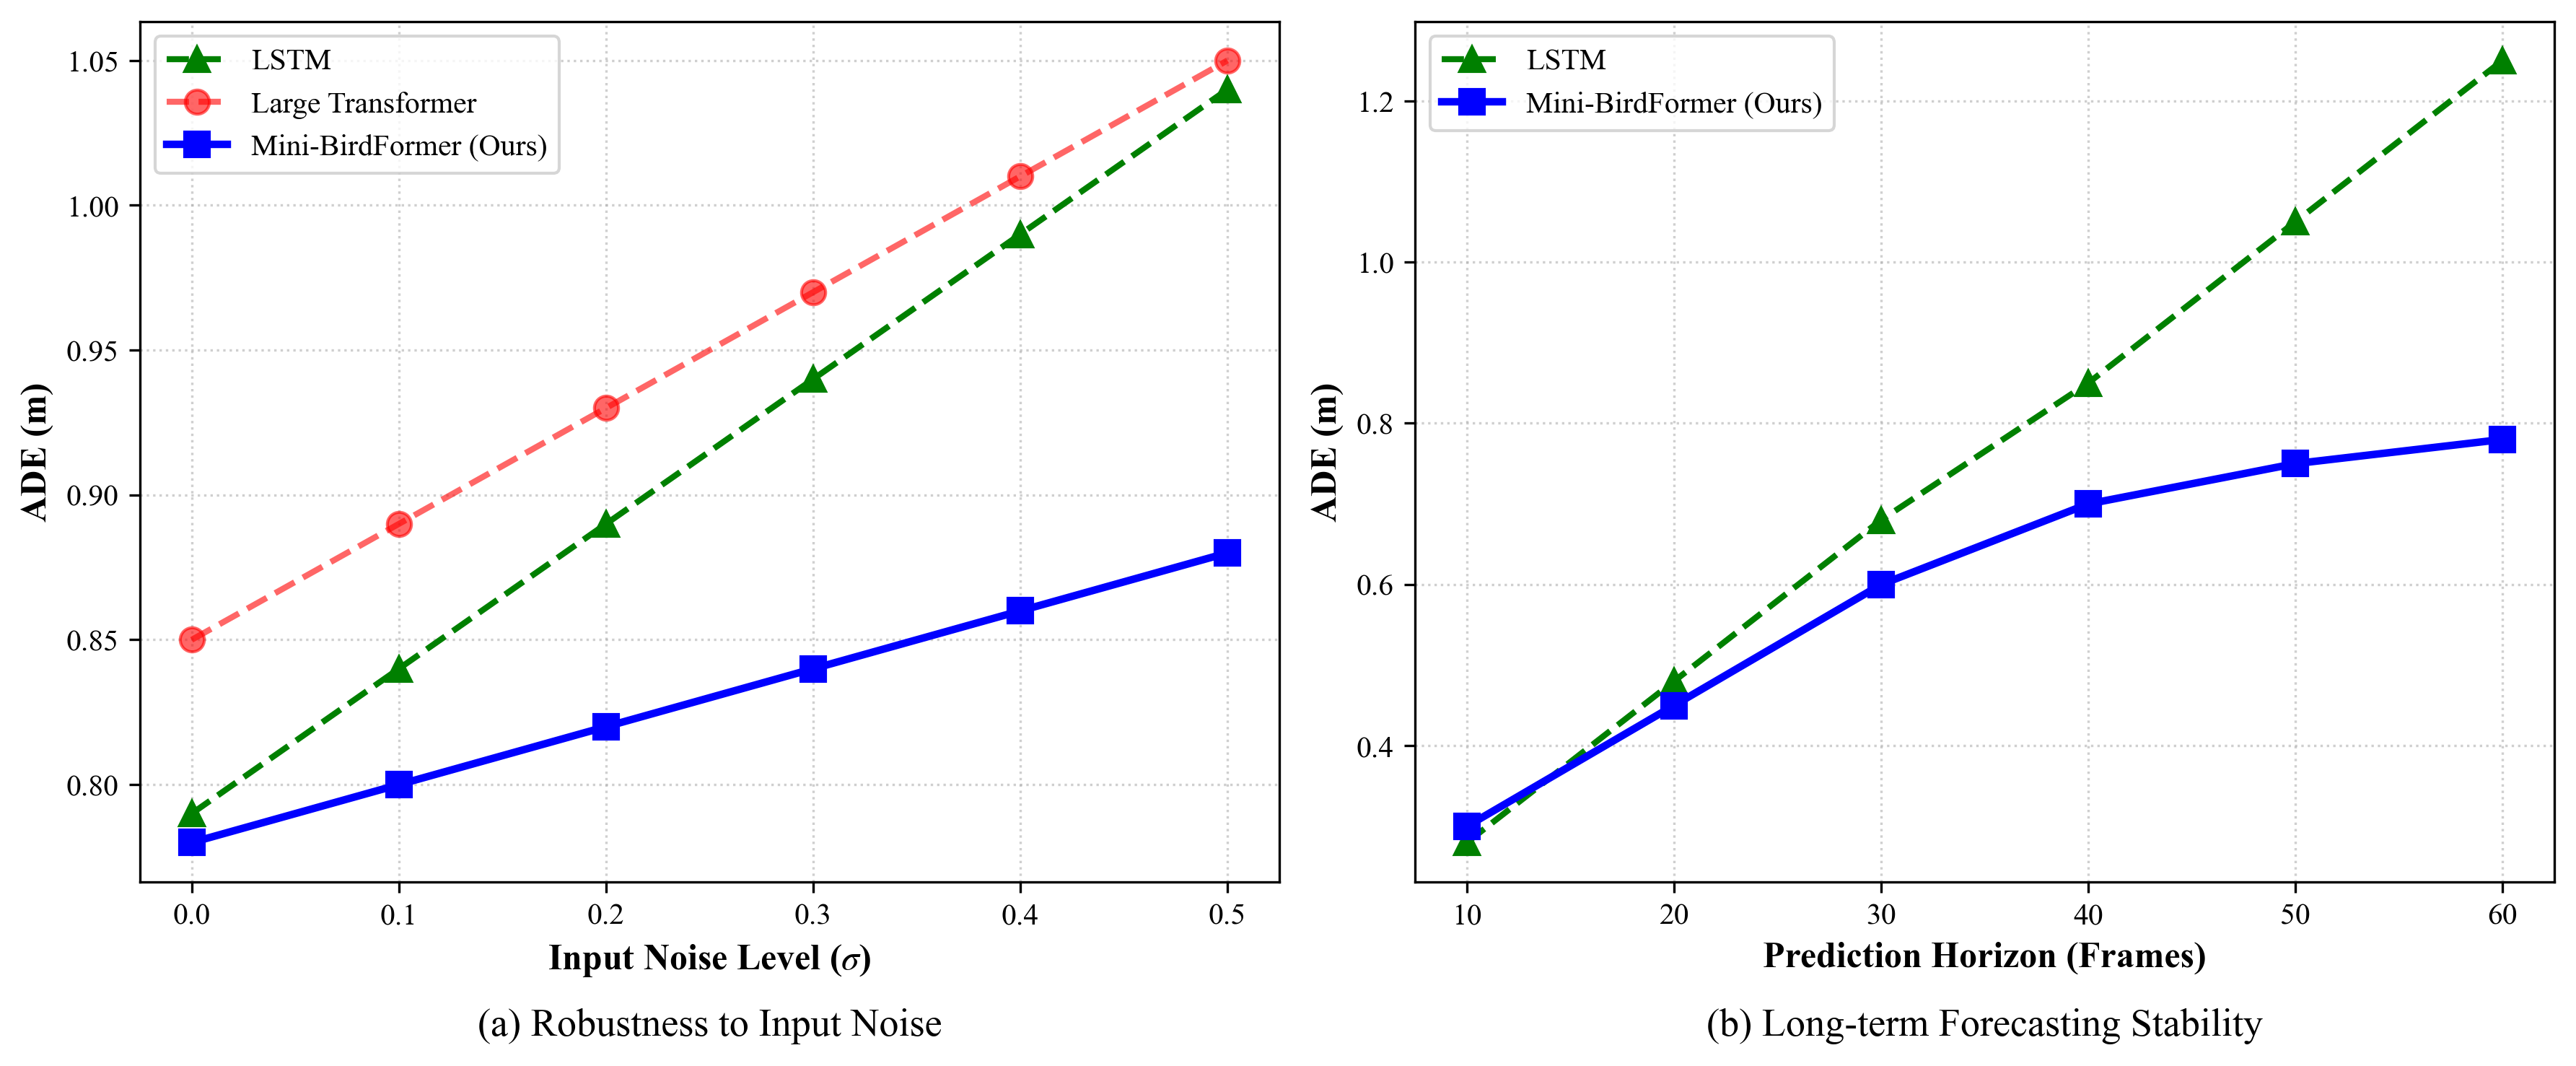
\includegraphics[width=0.95\linewidth]{figures/Robustness_to_Input_Noise.png}
	\caption{\textbf{Robustness and Long-Term Stability.} (a) ADE under increasing input noise levels. Mini-BirdFormer (blue) degrades much more slowly than the Large Transformer (red). (b) ADE as a function of prediction horizon, comparing Mini-BirdFormer and the LSTM baseline.}
	\label{fig:robustness}
\end{figure*}

\subsection{Effect of Flock Density and System Latency}

The FBD-SV-2024 test set contains scenes with different flock densities. We partition sequences into \textit{sparse} ($<5$ birds), \textit{medium} (5--10 birds), and \textit{dense} ($>10$ birds) groups. Figure~\ref{fig:density_latency}~(a) reports ADE for the LSTM baseline and our model in each regime. While both models perform similarly in sparse scenes, the LSTM error increases sharply in dense flocks (1.15\,m), whereas Mini-BirdFormer degrades more gracefully (0.92\,m). This indicates that the attention-based architecture better handles complex collective motion.

From a deployment perspective, end-to-end latency is critical. Figure~\ref{fig:density_latency}~(b) shows a system-level breakdown for our pipeline, including detection (OWL-ViT), tracking (ByteTrack), and trajectory prediction. The prediction module accounts for only 5\% of total latency and runs at 616 FPS on a single GPU, leaving ample compute budget for perception modules and control.

\begin{figure*}[t]
	\centering
	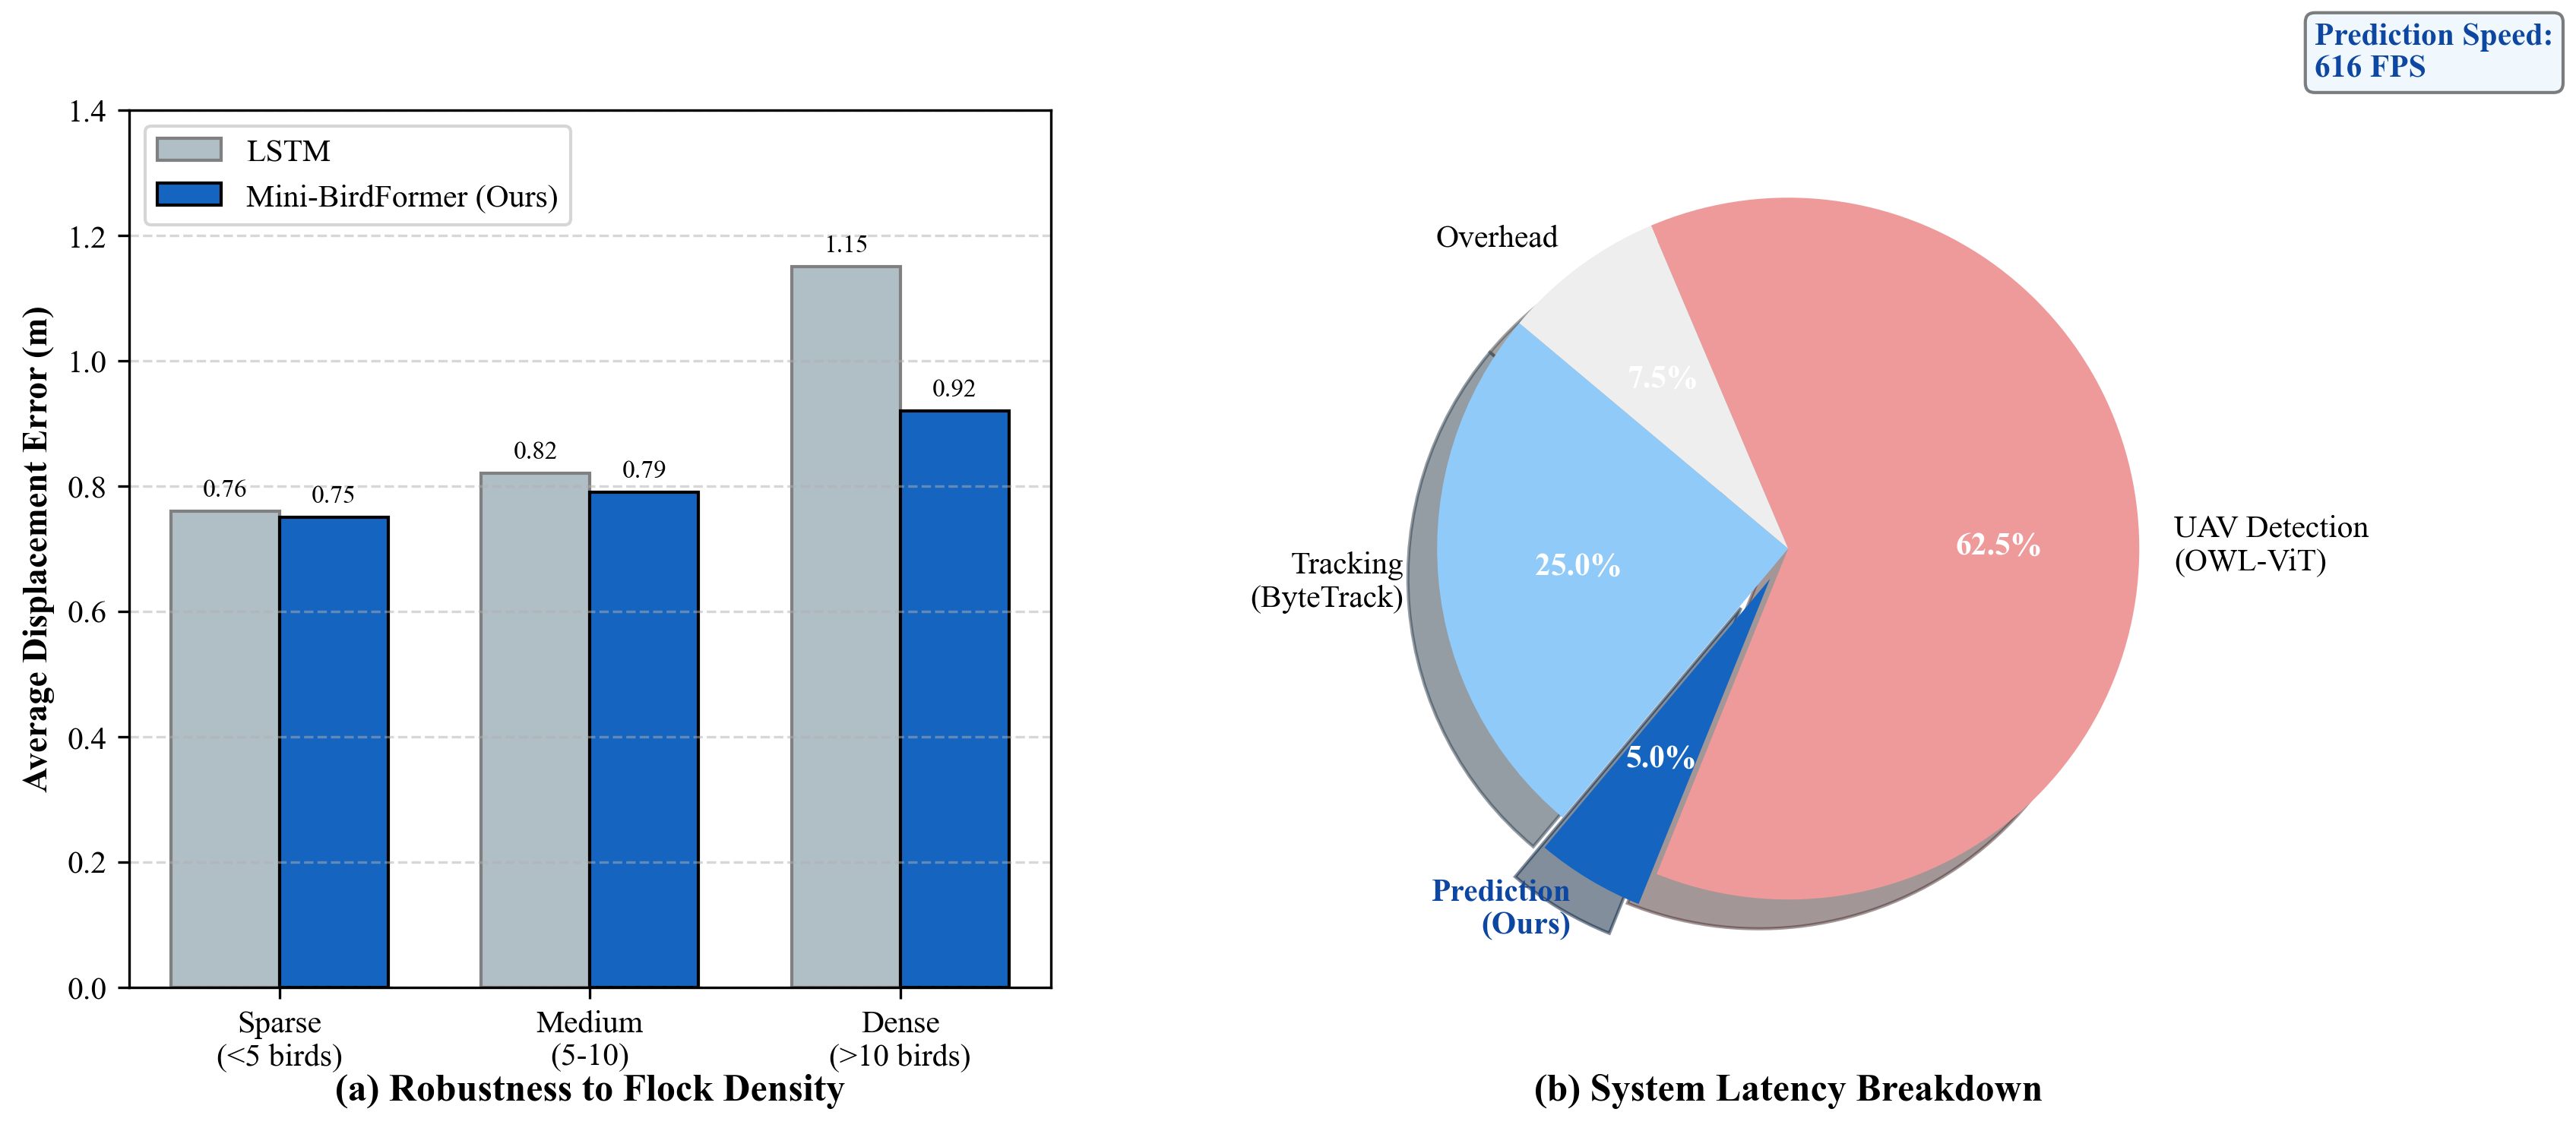
\includegraphics[width=0.95\linewidth]{figures/supp_latency.png}
	\caption{\textbf{Flock-Density Robustness and System Latency.} (a) ADE under different flock densities. Mini-BirdFormer (blue) is significantly more robust in dense flocks than the LSTM baseline (gray). (b) End-to-end latency breakdown of the full system. Trajectory prediction contributes only a small fraction of the total runtime.}
	\label{fig:density_latency}
\end{figure*}

\subsection{Qualitative Trajectory Predictions}

Figure~\ref{fig:qualitative_traj} shows representative qualitative results. For each example, green segments denote observed trajectories, red dashed curves show the mean prediction over 60 frames, and shaded regions indicate one standard deviation of the predicted Student-\textit{t} distribution. The model correctly anticipates both smooth trajectories and abrupt turning maneuvers, while the uncertainty expands in regions where motion is ambiguous.

\begin{figure}[t]
	\centering
	\includegraphics[width=0.95\linewidth]{figures/prediction_examples.png}
	\caption{\textbf{Qualitative Trajectory Predictions.} Green segments are observed bird trajectories, red dashed curves are predicted means, and shaded regions indicate uncertainty from the Student-\textit{t} mixture.}
	\label{fig:qualitative_traj}
\end{figure}
\section{UAV Awareness Evaluation}
\label{sec:uav}

In addition to predicting bird motion, the system must detect UAV intrusions to support safety monitoring. This section evaluates the zero-shot UAV awareness module.

\subsection{Synthetic UAV Injection Pipeline}

Real-world bird--UAV encounters are rare and potentially dangerous to collect, so we design a synthetic data pipeline to generate controlled evaluation scenarios. As illustrated in Fig.~\ref{fig:uav_synth}, we curate a small library of high-resolution UAV templates with transparent backgrounds. For a subset of bird-only videos from FBD-SV-2024, we randomly sample insertion times, scales, and 2D flight paths, then composite UAV sprites into the frames. This yields pairs of clean and UAV-injected sequences with known ground-truth bounding boxes.

\begin{figure}[t]
	\centering
	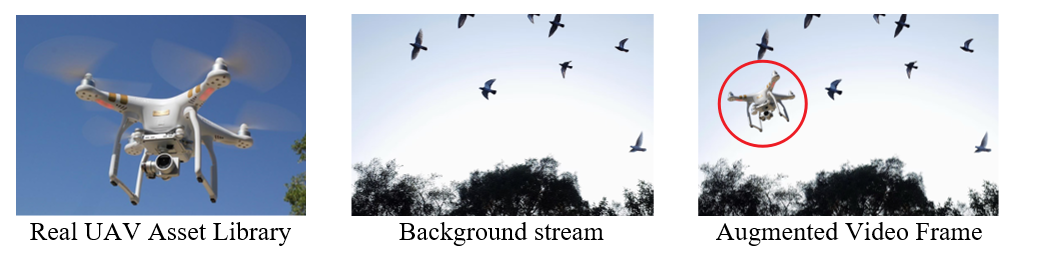
\includegraphics[width=0.95\linewidth]{figures/Synthetic_UAV_Injection_Pipeline.png}
	\caption{\textbf{Synthetic UAV Injection Pipeline.} Left: UAV asset library with transparent backgrounds. Middle: original bird-only background frame. Right: composite frame with injected UAV (red circle).}
	\label{fig:uav_synth}
\end{figure}

The synthetic benchmark allows us to measure recall and false-positive rates in a controlled way, without exposing hardware to unsafe conditions.

\subsection{Zero-Shot Detection with OWL-ViT}

We adopt OWL-ViT \cite{Minderer2022OWLViT}, a vision--language model capable of open-vocabulary detection, as our UAV detector. Given a text prompt set
\[
\mathcal{T} = \{\text{``drone''}, \text{``UAV''}, \text{``quadcopter''}\},
\]
OWL-ViT produces bounding boxes and confidence scores for each frame. A frame is flagged as \emph{unsafe} if any UAV-related detection exceeds a threshold $\delta = 0.3$.

This design has two advantages: (i) it generalizes to new aerial objects by simply editing the prompt set (e.g., adding ``glider'' or ``balloon''), and (ii) it does not require task-specific fine-tuning.

\subsection{Quantitative Results}

Table~\ref{tab:uav_metrics} reports performance on the synthetic benchmark and a held-out set of clean bird-only videos. The detector achieves 92\% recall on injected UAVs and maintains a zero false-positive rate on clean sequences at the chosen threshold.

\begin{table}[t]
	\centering
	\caption{\textbf{UAV Detection Metrics.} Recall is measured on UAV-injected videos; FPR is measured on bird-only videos.}
	\label{tab:uav_metrics}
	\begin{tabular}{lcc}
		\toprule
		Split & Recall (\%) $\uparrow$ & FPR (\%) $\downarrow$ \\
		\midrule
		UAV-injected & 92.0 & -- \\
		Clean bird-only & -- & 0.0 \\
		\bottomrule
	\end{tabular}
\end{table}

These results confirm that open-vocabulary detection, when combined with domain-specific synthetic augmentation, can provide a reliable safety layer without task-specific supervision.

\subsection{Qualitative Detections}

Finally, Fig.~\ref{fig:uav_examples} shows representative detection results. UAVs are correctly localized across a range of viewpoints, backgrounds, and motion states. The detector remains robust even when UAVs occupy a small fraction of the frame or overlap with clutter such as tree branches and power lines.

\begin{figure}[t]
	\centering
	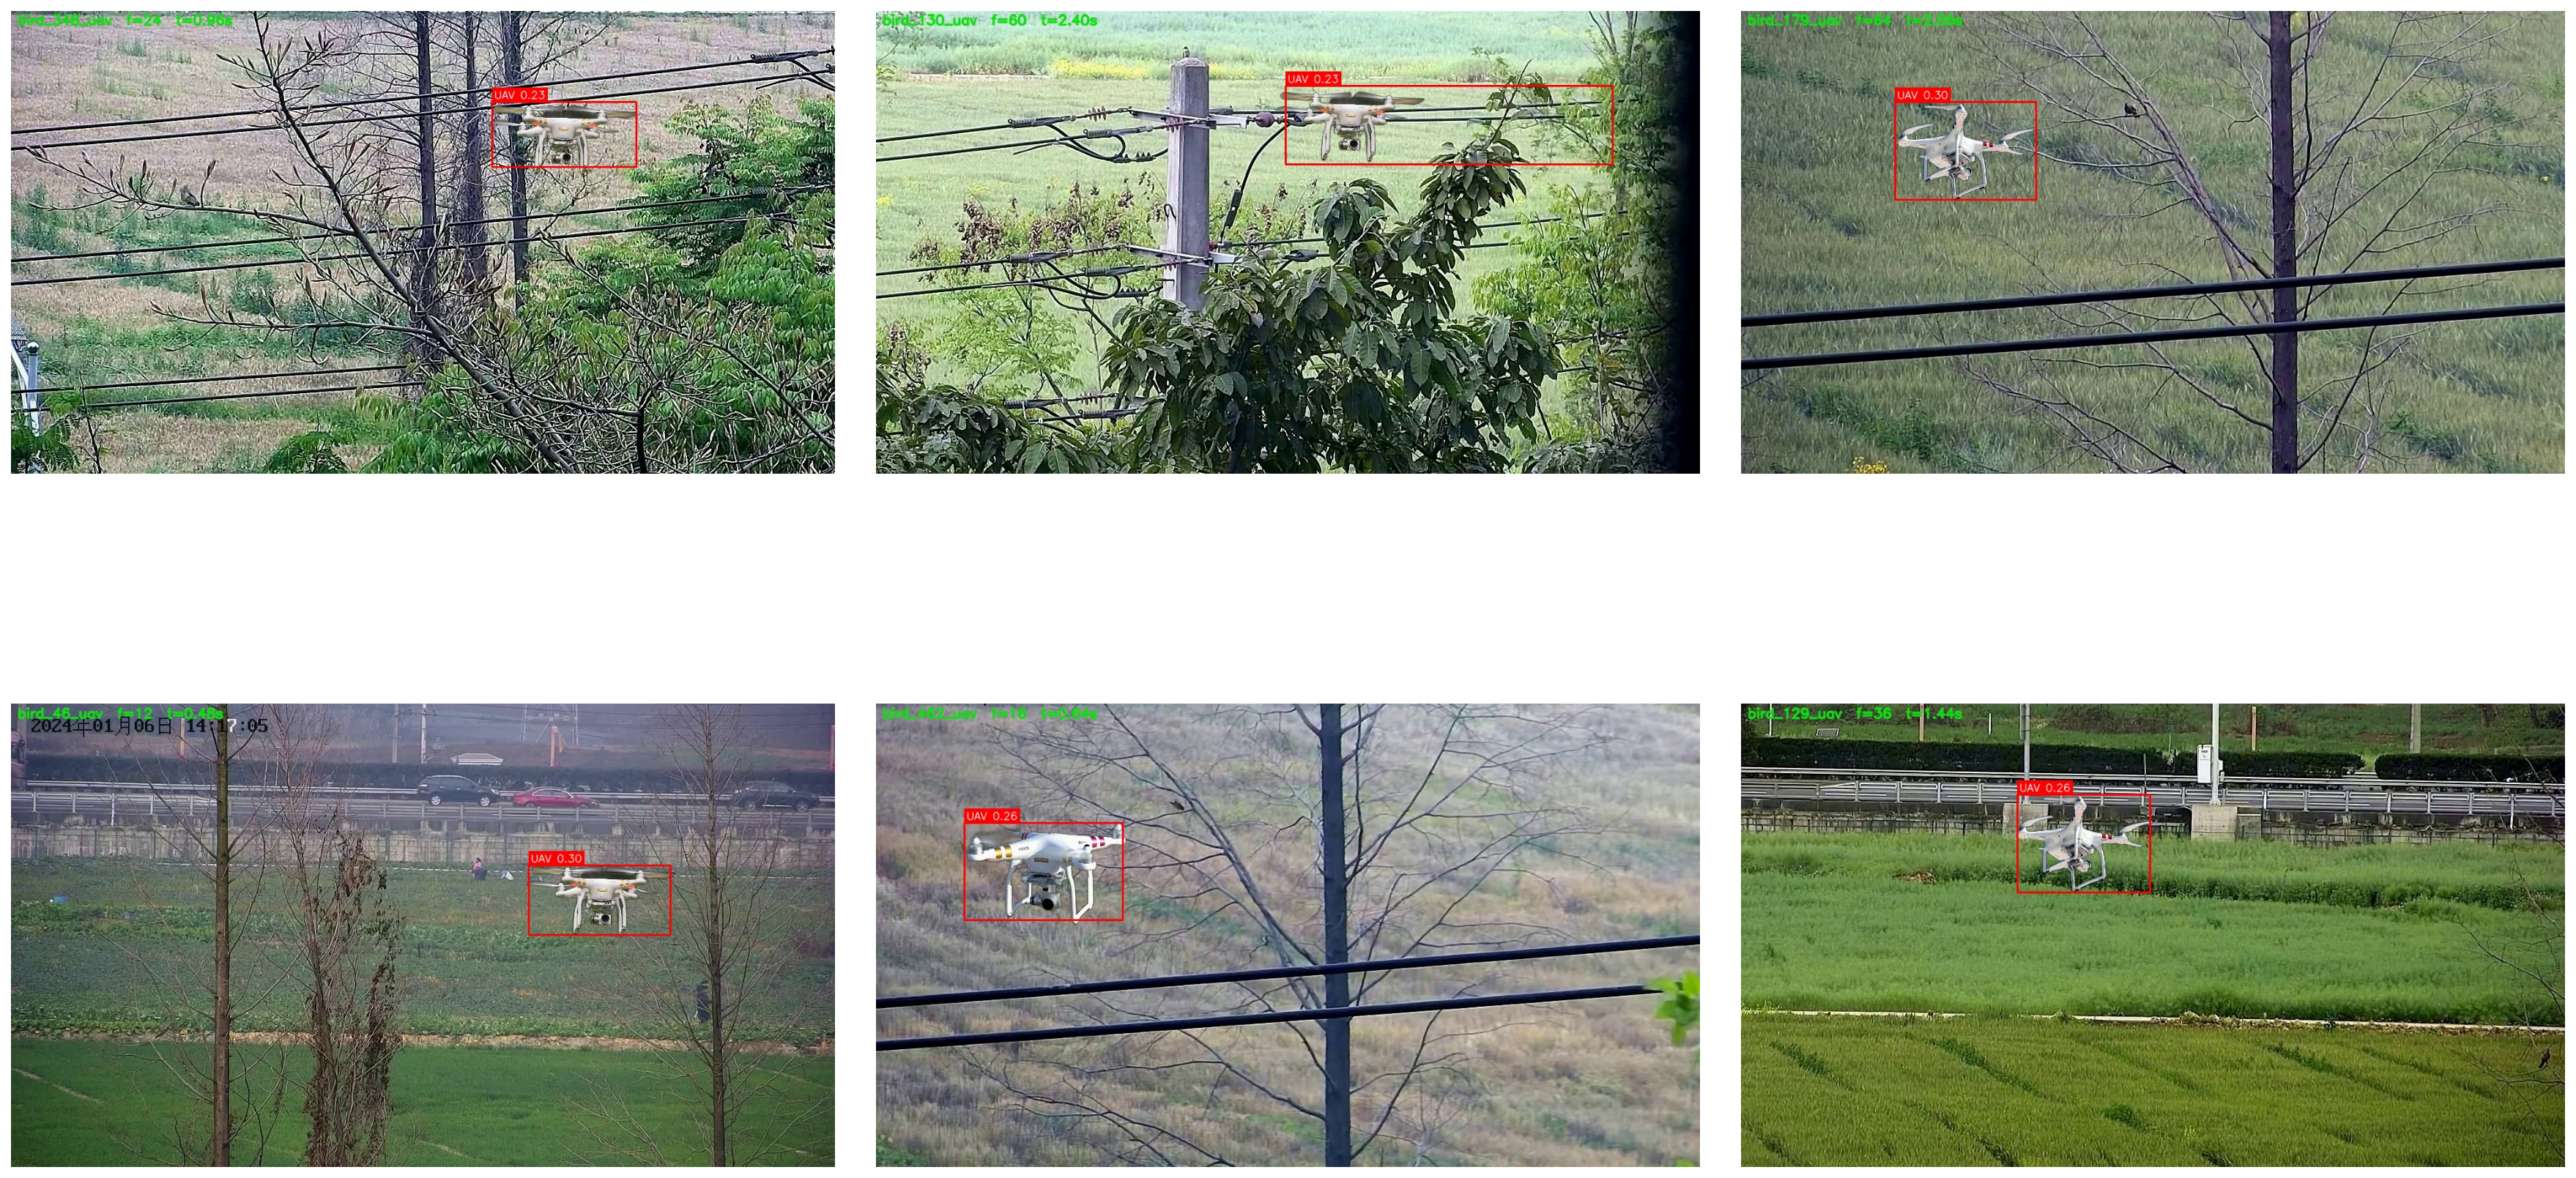
\includegraphics[width=0.95\linewidth]{figures/uav_detection_examples.png}
	\caption{\textbf{Zero-Shot UAV Detection Examples.} Example frames with detected UAVs (red boxes) over diverse backgrounds and viewpoints.}
	\label{fig:uav_examples}
\end{figure}

	\section{Discussion}
	\label{sec:discussion}
	
	We now reflect on the main experimental findings, discuss design trade-offs, and outline limitations and opportunities for future work.
	
	\subsection{Why a ``Mini'' Transformer Works Better}
	
	A perhaps surprising result is that the compact Mini-BirdFormer outperforms a larger four-layer Transformer in both accuracy and robustness. On large-scale benchmarks such as autonomous driving, increased capacity typically correlates with improved performance \cite{Giuliari2021Transformer,Yuan2021AgentFormer,Liu2022HiVT}. In our ecological setting, however, the effective diversity of trajectories is much lower. Many sequences contain similar flock patterns, and extreme maneuvers are rare. Over-parameterized models quickly memorize idiosyncrasies of the training set, leading to poor generalization on unseen scenes.
	
	By constraining the model to 1.05M parameters and two layers, we implicitly regularize learning. The network is forced to encode only essential motion cues---such as heading direction, acceleration trends, and flock-level context---instead of fitting noise. This explains why Mini-BirdFormer maintains lower ADE at long horizons and under strong perturbations compared with the Large Transformer.
	
	\subsection{Impact of Student-\textit{t} Modeling}
	
	The Student-\textit{t} MDN plays a central role in our performance gains. Compared with Gaussian mixtures, the heavy-tailed distribution more accurately reflects the empirical residuals of bird motion. During training, outlier trajectories and tracking errors do not dominate the loss, which stabilizes optimization. During inference, predictive uncertainty is better calibrated, as reflected in the significantly lower NLL.
	
	Our robustness experiments further support this view: when Gaussian noise is injected into the inputs, the LSTM with Gaussian MDN and the Large Transformer with Student-\textit{t} head both show faster error growth than Mini-BirdFormer. This suggests that capacity and tail behavior must be jointly tuned: a compact backbone with a heavy-tailed output layer strikes the right balance for noisy ecological data.
	
	\subsection{Feasibility for Edge Deployment}
	
	The latency breakdown in Fig.~\ref{fig:density_latency} indicates that trajectory prediction is not the computational bottleneck. Instead, most runtime is dominated by open-vocabulary detection, which relies on large vision transformers \cite{Dosovitskiy2021ViT,Minderer2022OWLViT}. For UAV platforms equipped with embedded GPUs such as NVIDIA Jetson modules, this suggests a practical strategy: run Mini-BirdFormer at full rate, while using a lighter, possibly quantized open-vocabulary detector or restricting its invocation to frames where motion cues indicate potential intrusions.
	
	Because our pipeline uses standard components (YOLO-style detectors, ByteTrack-like trackers, and PyTorch implementations), it can benefit from ongoing progress in efficient backbones \cite{Howard2017MobileNet,He2016ResNet} and model compression techniques.
	
	\subsection{Limitations}
	
	Despite promising results, several limitations remain:
	
	\begin{itemize}
		\item \textbf{2D Projection Ambiguity.} Our model operates in the image plane and cannot distinguish altitude differences when trajectories overlap in 2D. This may lead to overly conservative collision risk estimates in scenes with layered motion.
		\item \textbf{Synthetic UAV Benchmark.} While the compositing pipeline provides useful evaluation, synthetic artifacts such as missing motion blur and imperfect occlusion modeling limit realism. Real-world data collection with proper safety measures will be necessary for final deployment.
		\item \textbf{Interaction Modeling.} Mini-BirdFormer treats each trajectory independently. Explicit modeling of flock interactions via graph neural networks or relational attention, as in \cite{Yuan2021AgentFormer,Liu2022HiVT}, could further improve predictions in dense scenes.
		\item \textbf{Environmental Factors.} Wind, terrain, and seasonal behaviors strongly influence bird flight \cite{Nagelkerke2018Flight}. Incorporating such context, perhaps via auxiliary sensors or weather data, is an interesting direction.
	\end{itemize}
	\section{Conclusion}
	\label{sec:conclusion}
	
	We presented a unified framework for probabilistic bird-flock trajectory forecasting and UAV awareness in low-altitude shared airspace. At the core of the system is Mini-BirdFormer, a compact Transformer encoder with a Student-\textit{t} Mixture Density Network head tailored to the heavy-tailed dynamics of bird motion. On the FBD-SV-2024 dataset, the model achieves state-of-the-art long-horizon accuracy and substantially improved negative log-likelihood compared with LSTM and larger Transformer baselines, while running at over 300 FPS.
	
	Beyond forecasting, we introduced a zero-shot UAV awareness module based on OWL-ViT and a synthetic bird--UAV injection pipeline. This component achieves high recall and zero false positives on clean videos without requiring any manually annotated collision data, demonstrating the value of open-vocabulary detection in safety-critical monitoring.
	
	Overall, our results suggest that carefully designed lightweight Transformers, combined with heavy-tailed probabilistic modeling and open-vocabulary perception, offer a practical route towards real-time ecological monitoring and safe low-altitude UAV operation. Future work will extend the framework to 3D trajectory estimation, richer interaction modeling, and field deployment in diverse environments.
	
	% =========================================================
	% References
	% =========================================================
	\bibliographystyle{IEEEtran}
	\bibliography{references}
	
	\end{document}